\begin{center}
    \Large{\textbf{Теоретична частина}}    
\end{center}

\vspace{1mm}

Хвильова природа світла найбільш яскраво спостерігаєтьтся в явищі
дифракції, тобто в явищі огинання світлом перешкод(екранів, отворів).

\begin{wrapfigure}{r}{0.5\textwidth}    
    \centering
    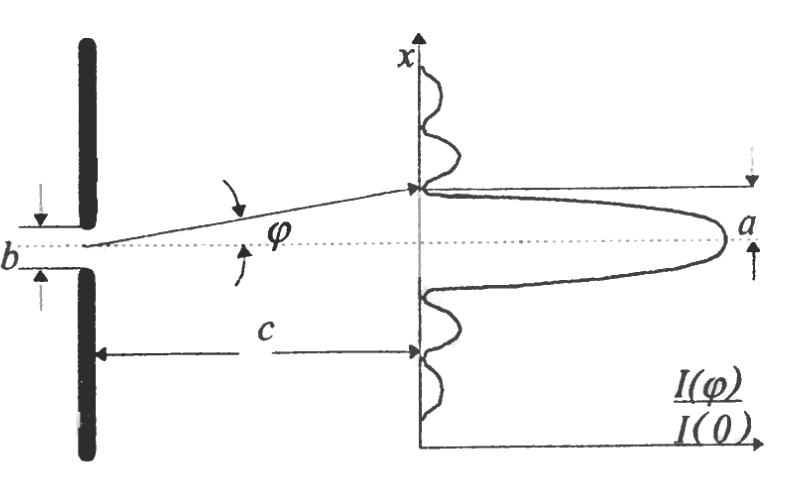
\includegraphics[width=.5\textwidth]{assets/diffraction.png}
    \caption{Дифракція в паралельних променях}
\end{wrapfigure}

Розглянемо пучок паралельних монохроматичних променів з 
довжиною хвилі $\lambda$, що падають на щілину шириною $b$(рис. 1).
Площину щілини можна розбити на ряд вузеньких паралельних
смужок однакової ширини. Кожну з таких смужок будемо розглядати
як джерело хвиль, причому фази і амлітуди всіх цих хвиль однакові,
оскільки за нормального падіння площина щілини збігається 
з поверхнею хвилі. Для розрахунку інтенсивності в різних
напрямках напишемо вираз хвилі, що посилає кожний елемент хвилі
товщини $dx$, і підсумуємо дію всіх елементів. Амплітуда хвилі,
зумовлена таким елементом, очевидно, пропорційна $dx$,
а відповідне збурення дорівнює

\begin{equation} \label{eq:1}
    dE = \frac{A_0}{b} dx \cdot e^{i \omega t},
\end{equation}

де $\omega$ - циклічна частота, $A_0$ - сумарна амплітуда
хвилі, що посилає вся щілина. В напрямку спостереження всі
елементарні хвилі будуть мати однакову фазу, і тому результуюча амплітуда
буде $E=A_0$. Для хвиль, що розповсюджуються під кутом $\varphi$
до напрямку спостереження, треба врахувати різницю фаз, яка 
характеризує хвилі, що приходять від різних елементів щілини.
З геометричних міркувань зрозуміло, що різниця ходу для елементу,
що знаходиться на відстані $x$ від краю щілини, дорівнює $x\sin{\varphi}$.
Відповідне елементарне світлове збурення

\begin{equation} \label{eq:2}
    dE = \frac{A_0}{b}dx \cdot e^{i(\omega t - kx \sin{\varphi})},
\end{equation}

де $k = \frac{2 \pi}{\lambda}$ - хвильове число. Отже, результуюче збурення

\begin{equation} \label{eq:3}
    E = \int\limits_{\frac{-b}{2}}^{\frac{b}{2}} dE = 
    \int\limits_{\frac{-b}{2}}^{\frac{b}{2}} \frac{A_0}{b}dx \cdot e^{i(\omega t - kx \sin{\varphi})} dx = 
    A_0 \frac{\sin{( \frac{bk}{2} \sin{\varphi} )}}{ \frac{bk}{2} \sin{\varphi} } e^{i \omega x},
\end{equation}

а інтенсивність у вказаному напрямку

\begin{equation} \label{eq:4}
    I(\varphi) = I(0) \left[ \frac{\sin{( \frac{bk}{2} \sin{\varphi} )}}{ \frac{bk}{2} \sin{\varphi} } \right]^2 = 
    I(0) \left[ \frac{\sin{u}}{u} \right]^2, \; u = \frac{bk \sin{\varphi}}{2}
\end{equation}

Формулу \ref{eq:4} називають формулою Кірхгоффа. З цієї формули видно,
що за певних кутів спостереження $\varphi_n$, а саме

\begin{equation} \label{eq:5}
    \sin{\varphi_n} = \frac{n \lambda}{b}, \; n = 1,2, \cdots
\end{equation}

інтенсивність дорівнює нулю, що відповідає темним смугам на екрані.
Крім того, між мінімумами знаходяться максимуми. Їх положення
визначається умовою рівності нулю похідної від \ref{eq:3}:

\begin{equation} \label{eq:6}
    \frac{d \left( \frac{\sin{u}}{u} \right) }{du} = 0,
\end{equation}

де $u$ - розв'язок трансцендентного рівняння

\begin{equation} \label{eq:7}
    \tan{u} = u 
\end{equation}

для перших трьох максимумів буде:

\begin{equation}  \label{eq:7A}
    \begin{gathered}
        \frac{bk}{2}\sin{\varphi} = 0, \;
        \frac{bk}{2}\sin{\varphi} = 1.43 \pi, \;
        \frac{bk}{2}\sin{\varphi} = 2.46 \pi \\
        \frac{bk}{2}\sin{\varphi} = 3.47 \pi, \;
        \frac{bk}{2}\sin{\varphi} = 4.47 \pi
    \end{gathered}    
    \tag{7A}
\end{equation}

Величина інтенсивності в цих максимумах тим менша, чим більший
номер максимуму. Відношення інтенсивністей наближено можна виразити рядом:

\begin{equation} \label{eq:8}
    1 : \left( \frac{2}{3 \pi} \right)^2 : 
    \left( \frac{2}{5 \pi} \right)^2 : 
    \left( \frac{2}{7 \pi} \right)^2 : \cdots
\end{equation}


Таким чином, за умов коли паралельний монохроматичний
когерентний світловий промінь проходить через щілину, на екрані
розташованому за щілиною виникає дифракційна картина з головними
та додатковими максимумами.

\begin{wrapfigure}{r}{0.5\textwidth}    
    \centering
    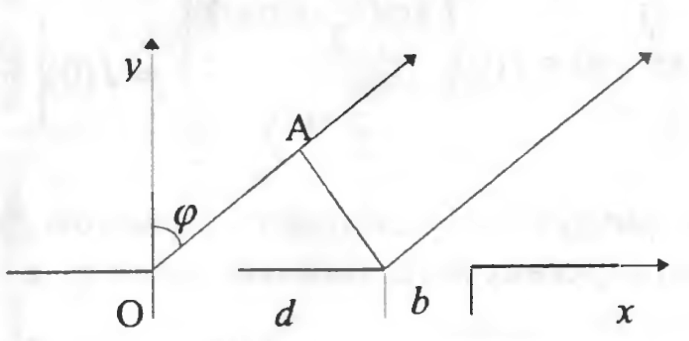
\includegraphics[width=.5\textwidth]{assets/diffraction_in_two.png}
    \caption{Дифракція від двох щилин}
\end{wrapfigure}

Розглянемо тепер дифракцію від двох паралельних щілин.
Дві дифракційні картини від кожної з щілин накладуться одна на одну.
При цьому треба прийняти до уваги взаємну інтерференцію
хвиль, що ідуть від першої та другої щілини. Очевидно,
що в тих напрямках, куди ні одна з щілин не посилаж світла,
не буде світла і при двох щілинах. Тобто, мінімуми інтенсивності
залишаються на старих місцях Окрім того, з'являються нові
мінімуми, оскільки існують напрямки, в яких коливання від
відповідних точок двох щілин взаємно знищуються. Це напрямки, для яких
різниця ходу від відповідних точок двох щілин становить 
$\frac{\lambda}{2}, \frac{3 \lambda}{2} \cdots$. Як видно
з рис. 2 такі напрямки визначаються умовою

\begin{equation} \label{eq:9}
    OA = d \cdot \sin{\varphi} = \frac{1}{2} \lambda, \frac{3}{2} \lambda, \cdots
\end{equation}

В напрямках, що визначаються умовами 

\begin{equation} \label{eq:10}
    d \cdot \sin{\varphi} = \lambda, 2\lambda, \cdots
\end{equation}

дія щілин підсилюється, а отже в цих напрямках з'являються
максимуми. Узагальнюючи вищесказане можна зробити висновок,
що повна дифракційна картина від двох щілин визначається такими
умовами:

\begin{equation} \label{eq:11}
    \begin{aligned}
        \text{колишні мінімуми} \; b \cdot \sin{\varphi} =& \lambda, \; 2 \lambda, \; 3 \lambda, \cdots \\
        \text{додаткові мінімуми} \; d \cdot \sin{\varphi} =& \frac{1}{2} \lambda, \; \frac{3}{2} \lambda, \; \frac{5}{2} \lambda \cdots \\
        \text{головні максимуми} \; b \cdot \sin{\varphi} =& 0, \; \lambda, \; 2 \lambda, \cdots \\
    \end{aligned}
\end{equation}

Міркування, наведені для двоз щілин, залишаються слушними для
випадку $N$ щілин, тобто дифракційної решітки - екрана з
регулярною структурою, наприклад довгими і вузькими щілинами
з паралельними краями. Додаткові мінімуми з'являються за рахунок
інтерференції випромінювання від першої щілини з випромінюванням
від другої, третьої і далі до $(N-1)$. Умова \ref{eq:11} перепишеться як:

\begin{equation} \label{eq:12}
    \begin{aligned}
        \text{колишні мінімуми} \; b \cdot \sin{\varphi} =& \lambda, \; 2 \lambda, \; 3 \lambda, \cdots \\
        \text{додаткові мінімуми} \; d \cdot \sin{\varphi} =& \frac{1}{N} \lambda, \; \frac{2}{N} \lambda ,\cdots, \; \frac{N-1}{N} \lambda \cdots \\
        \text{головні максимуми} \; b \cdot \sin{\varphi} =& 0, \; \lambda, \; 2 \lambda, \cdots \\
    \end{aligned}
\end{equation}


Отримаємо аналітичний вираз для розподілу інтенсивності від $N$ щілин.
Напруженість поля від першої щілини в напрямку $\varphi$ 
описується формулою \ref{eq:3}. Для хвиль, що дифрагують 
на другій, третій і далі щілині, напруженість буде відрізняться
фазовим множником:

\begin{equation} \label{eq:13}
    E_N(\varphi) = E_1(\varphi) \cdot e^{i(N-1)\delta}, \;
    \delta = \frac{2 \pi d}{\lambda} \sin{\varphi}
\end{equation}

Тоді, результуючі напруженість та інтенсивність від усіх щілин буде:

\begin{equation} \label{eq:14}
    \begin{gathered}
        E_P(\varphi) = E_1(\varphi) \left[ 1 + e^{i\delta} + e^{2 i\delta} + \cdots + e^{i (N-1) \delta} \right] \\
        I(\varphi) = E \cdot E^{*} = I(\varphi) \frac{\sin^2{\frac{N\delta}{2}}}{\sin^2{\frac{\delta}{2}}}
    \end{gathered}
\end{equation}


З \ref{eq:14} видно, що для напрямків, в яких різниця фаз
$\frac{\delta}{2} = m \pi (m = 0, \pm 1, \pm 2, \cdots)$
інтенсивність випромінювання зростає у $N^2$ разів, тобто
ці напрямки відповідають головним максимумами в дифракційній
картині, як і витікає з умов \ref{eq:12}. Ширина головних максимумів
$\varepsilon$ на половині висоти визначається з умови

$$ \dfrac{ \sin^2{\frac{N \delta_{\frac{1}{2}}}{2}} }
{\sin^2{\frac{\delta_{\frac{1}{2}}}{2}}} = \frac{N^2}{2}, $$ 

де $ \delta_{\frac{1}{2}} = m \pi \pm \frac{\varepsilon}{2} $
Рішення цього трансцендентного рівняння дає
$ \varepsilon = \frac{5.6}{N} $. Щільність дифракційної картини
- відношення відстані між головними максимумами до Їх
ширини - буде дорівнювати:

\begin{equation} \label{eq:15}
    F = \frac{\Delta \delta}{\varepsilon} = 1.13N
\end{equation}

Тобто різкість дифракційної картини пропорційна загальній
кількості щілин(штрихів) дифракційної решітки.


Розглянемо тепер явище дифракції з точки зору кванотової
механіки. Згідно з принципом невизначенності Гейзенберга
неможливо одночасне точне визначення значень спряжених змінних,
таких як координата $x$ та імпульс $p$ в один і той же
момент часу, або в аналітичному вигляді

\begin{equation} \label{eq:16}
    \Delta x \cdot \Delta p \ge \frac{\hbar}{4 \pi}
\end{equation}

де $\Delta x$, $\Delta p$ - похибки у визначенні координати
та імпульсу, відповідно, $\hbar = 6.6262 \cdot 10^{-34}$ Дж $\cdot$ сек -
стала Планка.


Розглянемо, для прикладу, сукупність фотонів, ймовірність
знаходження яких у просторі описується функцією $f_x$, 
а розподіл імпульсів - функцією $f_p$ $d$. Якщо фотони
проходять крізь щілину завширшки $d$, то поперек щілини
їх координата визначена з точністю

\begin{equation} \label{eq:17}
    \Delta x = d
\end{equation}

Густина ймовірності для відповідної компоненти імпульсу
визначається розподілом інтенсивності в дифракційній картині.
Справді, інтенсивність пропорційна кількості фотонів, що 
прийшли в задане місце протягом певного часу, отже,
невизначенність імпульсу пропорційна відстані між
мінімумами дифракційної картини, тобто

\begin{equation} \label{eq:18}
    \Delta p_x = p_0 \sin{\varphi},
\end{equation}

де $p_0$ - початковий імпульс. Застосовуючи співвідношення
Де-Бройля $p = \frac{h}{\lambda}$ і підставляючи відстань між
мінімумами з формули \ref{eq:12} отримуємо

\begin{equation} \label{eq:19}
    \Delta p_x = \frac{h}{\lambda} \sin{\varphi} = \frac{h}{d}
\end{equation}

Порівнюючи \ref{eq:17} та \ref{eq:19} бачимо, що користуючись
щілиною для визначення координати фотона(локалізації його
у просторі з точністю $d$), ми спотворюємо точність визначення
імпульсу таким чином, що

$$ \Delta x \Delta p = h $$

Отже, дифракція може розглядатися як один з проявів
фундаментального принципу невизначенності \ref{eq:16}.
%\begin{figure}[h]    
%    \centering
%    \includegraphics[width=.7\textwidth]{assets/filename }
%    \caption{Підпис}
%\end{figure}